\documentclass{article}

\usepackage{tikz} 
\usetikzlibrary{automata, positioning, arrows} 

\usepackage{amsthm}
\usepackage{amsfonts}
\usepackage{amsmath}
\usepackage{amssymb}
\usepackage{fullpage}
\usepackage{color}
\usepackage{parskip}
\usepackage{hyperref}
  \hypersetup{
    colorlinks = true,
    urlcolor = blue,       % color of external links using \href
    linkcolor= blue,       % color of internal links 
    citecolor= blue,       % color of links to bibliography
    filecolor= blue,        % color of file links
    }
    
\usepackage{listings}
\usepackage[utf8]{inputenc}                                                    
\usepackage[T1]{fontenc}                                                       

\definecolor{dkgreen}{rgb}{0,0.6,0}
\definecolor{gray}{rgb}{0.5,0.5,0.5}
\definecolor{mauve}{rgb}{0.58,0,0.82}

\lstset{frame=tb,
  language=haskell,
  aboveskip=3mm,
  belowskip=3mm,
  showstringspaces=false,
  columns=flexible,
  basicstyle={\small\ttfamily},
  numbers=none,
  numberstyle=\tiny\color{gray},
  keywordstyle=\color{blue},
  commentstyle=\color{dkgreen},
  stringstyle=\color{mauve},
  breaklines=true,
  breakatwhitespace=true,
  tabsize=3
}

\newtheoremstyle{theorem}
  {\topsep}   % ABOVESPACE
  {\topsep}   % BELOWSPACE
  {\itshape\/}  % BODYFONT
  {0pt}       % INDENT (empty value is the same as 0pt)
  {\bfseries} % HEADFONT
  {.}         % HEADPUNCT
  {5pt plus 1pt minus 1pt} % HEADSPACE
  {}          % CUSTOM-HEAD-SPEC
\theoremstyle{theorem} 
   \newtheorem{theorem}{Theorem}[section]
   \newtheorem{corollary}[theorem]{Corollary}
   \newtheorem{lemma}[theorem]{Lemma}
   \newtheorem{proposition}[theorem]{Proposition}
\theoremstyle{definition}
   \newtheorem{definition}[theorem]{Definition}
   \newtheorem{example}[theorem]{Example}
\theoremstyle{remark}    
  \newtheorem{remark}[theorem]{Remark}

\title{CPSC-354 Report}
\author{Ethan Tapia  \\ Chapman University}

\date{\today} 

\begin{document}

\maketitle

\begin{abstract}
\end{abstract}

\setcounter{tocdepth}{3}
\tableofcontents

\section{Introduction}\label{intro}

\section{Week by Week}\label{homework}

\subsection{Week 1}

\textbf{Lecture Summary}

We introduced \emph{formal systems} and worked with Hofstadter’s MIU-system as a rule–based rewriting game.  
Alphabet: $\Sigma=\{M,I,U\}$.  
Axiom (start string): $MI$.  
Production rules:
\begin{enumerate}
    \item[\textbf{(R1)}] If a string ends in $I$, append $U$: $xI \Rightarrow xIU$.
    \item[\textbf{(R2)}] If a string is $Mx$, duplicate $x$: $Mx \Rightarrow Mxx$.
    \item[\textbf{(R3)}] Replace any $III$ by $U$: $xIIIy \Rightarrow xUy$.
    \item[\textbf{(R4)}] Delete any $UU$: $xUUy \Rightarrow xy$.
\end{enumerate}
Key idea: reason about \emph{invariants} that rules preserve, instead of searching blindly through derivations.

\bigskip
\textbf{Homework: The MU-puzzle}

\begin{definition}[I–count and residue]
For a string $w$, let $\#_I(w)$ be the number of $I$’s in $w$, and define the residue
\[
\varphi(w) \;=\; \#_I(w) \bmod 3 \in \{0,1,2\}.
\]
\end{definition}

\begin{lemma}[Effect of each rule on $\#_I$]\label{lem:rule-effects}
For any string $w$:
\begin{enumerate}
    \item \textbf{(R1)} and \textbf{(R4)} do not change $\#_I$.
    \item \textbf{(R2)} doubles the number of $I$’s \emph{after} the initial $M$, so $\varphi$ is multiplied by $2$ modulo $3$.
    \item \textbf{(R3)} decreases $\#_I$ by $3$, so $\varphi$ is unchanged.
\end{enumerate}
\end{lemma}

\begin{proposition}[Invariant modulo $3$]\label{prop:invariant}
Every string derivable from $MI$ has $\varphi\in\{1,2\}$. In particular, no derivable string has $\varphi=0$.
\end{proposition}

\begin{proof}
We use induction on the length of a derivation from $MI$.

\emph{Base.} $\varphi(MI)=1$.

\emph{Step.} Assume $\varphi\in\{1,2\}$ for some derivable $w$.  
By Lemma~\ref{lem:rule-effects}, rules (R1), (R3), and (R4) keep $\varphi$ unchanged, and rule (R2) maps $1\leftrightarrow 2$ modulo $3$. None of these operations yields $0$ from a value in $\{1,2\}$. Therefore the next string also has $\varphi\in\{1,2\}$.
\end{proof}

\begin{theorem}[MU is unreachable]
\label{thm:mu-unreachable}
$MU$ cannot be derived from $MI$ in the MIU-system.
\end{theorem}

\begin{proof}
$MU$ contains zero $I$’s, hence $\varphi(MU)=0$. By Proposition~\ref{prop:invariant}, every derivable string has residue $1$ or $2$. Thus $MU$ is not derivable.
\end{proof}

\textit{Conclusion.} Starting from $MI$ we can toggle the residue $1\leftrightarrow 2$ with (R2) and otherwise keep it fixed with (R1), (R3), (R4). We never reach residue $0$, so no sequence of legal rule applications yields $MU$.

\begin{center}
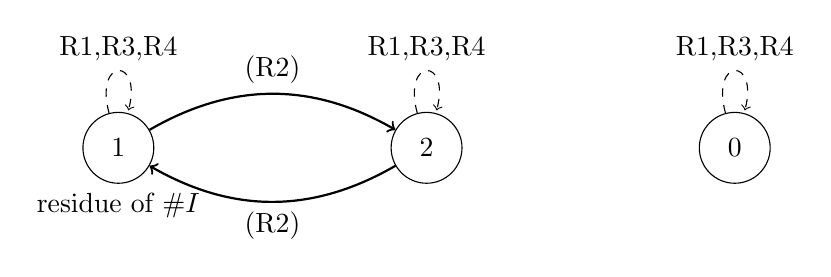
\begin{tikzpicture}[node distance=3cm, auto]
  \tikzstyle{state}=[circle,draw,minimum size=9mm]
  \node[state, label=below:{residue of $\#I$}] (Z1) {1};
  \node[state, right=of Z1] (Z2) {2};
  \node[state, right=of Z2] (Z0) {0};
  \path[->, thick]
    (Z1) edge[bend left] node[above]{(R2)} (Z2)
    (Z2) edge[bend left] node[below]{(R2)} (Z1);
  \path[->, dashed]
    (Z1) edge[loop above] node{R1,R3,R4} ()
    (Z2) edge[loop above] node{R1,R3,R4} ()
    (Z0) edge[loop above] node{R1,R3,R4} ();

\end{tikzpicture}
\end{center}
\textbf{Question:} If the MU-puzzle shows that some goals are unreachable due to invariants (like the mod-3 property of I’s), how does this idea connect to undecidability in programming languages?

\section{Essay}

\section{Evidence of Participation}

\section{Conclusion}\label{conclusion}

\begin{thebibliography}{99}
\bibitem[BLA]{bla} Author, \href{https://en.wikipedia.org/wiki/LaTeX}{Title}, Publisher, Year.
\end{thebibliography}

\end{document}
